\documentclass{article}
\usepackage{listings}
\usepackage[utf8]{inputenc}
\usepackage{ amssymb }
\usepackage{amsfonts}
\usepackage{graphicx}
\usepackage{color}
\definecolor{dkgreen}{rgb}{0,0.6,0}
\definecolor{gray}{rgb}{0.5,0.5,0.5}
\definecolor{mauve}{rgb}{0.58,0,0.82}

\title{Sistemas Distribuidos y Verificación \\ Tarea 10}
\author{Fabián Romero Jiménez}
\date{}
\begin{document}

\maketitle

\begin{enumerate}

\item[\bf{Problema 1}] Hacer un resumen de a lo más una cuartilla de {\it Don’t Settle for Eventual Consistency}

\item[\bf{Respuesta}]
En este artículo, primero se explica la importancia de tener bases de datos distribuidas en muchas localidades en el mundo (geo-replicación), pues para servicios disponibles en todo el mundo, como Facebook, disminuye la latencia al poder dar datos desde el centro de datos mas cercano, también al tener los datos en multiples lugares, la pérdida de datos de un centro de datos no implica la perdida de datos en el sistema, ni siquiera la interrupción del servicio, pues otro centro de datos, puede responder las peticiones.\\

El problema asociado con la geo-replicación, es el famoso teorema $CAP$ donde se muestra que en un sistema distribuido es imposible tener simultaneamente consistencia, disponibilidad y tolerancia a particiones. Por lo tanto, en un servicio distribuido la solución es debilitar al menos una de esas tres características, comunmente, si no se trata de dinero, la característica que se debilita es la tolerancia a particiones.\\

Una solución común y popular es el uso de sistemas ``eventualmente consistentes'', los cuales aseguran que los datos de dos centros de datos, eventualmente serán los mismos. Aparentemente es una debilitación satisfactoria de la tolerancia a particiones.\\

Sin embargo, consistencia eventual, solo se refiere a los datos como conjunto y no a la secuencialidad de los mismos, así, es completamente posible y esperado que usando solamante consistencia eventual se tengan secuencias que creen efectos indeseados, es decir, si la semantica de la información depende de su secuencia, p ej. si alguien anuncia una noticia buena y una mala, y como respuesta recibe felicitación por la buena y condolencia por la mala demostrando empatía, cambiando el orden de la respuestas, puede entenderse justo en el sentido opuesto.\\

Así que en el artículo se propone debilitar la tolerancia a particiones, pero no tanto como consistencia eventual, sino en algo que llaman ``consistencia causal'', la idea es que las actualizaciones que un centro de datos propaga a otros, sucedan en el mismo orden que en el centro de datos original. Aparentemente esto sería mucho mas costoso que la consistencia eventual, pues mucha comunicación extra debe de tomarse en cuenta para asegurar la causalidad de los eventos. También se debe retrasar la aplicación de las operaciones de escritura hasta que todas las operaciones anteriores en orden causal hayan tomado efecto.\\

Pero en pruebas efectuadas por los investigadores muestran que la perdida de desempeño comparado con sistemas de consistencia eventual (en este caso comparan con el muy popular manejador distribuido de datos apache Cassandra ) y el desempeño comparativo fue de aproximadamante $96\%$, es decir, escencialmente indistinguible, pero es muy ventajoso en el sentido de corrección semántica, haciendo de este enfoque una clara mejora sobre ``consistencia eventual''.


\item[\bf{Problema 2}] En la figura se muestra una historia para tres procesos, cada línea corresponde a un proceso diferente. Los tres procesos trabajan sobre una pila s. Este objeto tiene dos métodos:\\
\begin{itemize}
\item[{s.top(i)}] que indica que el elemento $i$ está en la casilla superior de la pila, pero no elimina al elemento $i$
\item[{s.push(i)}] que pone el elemento $i$ en la casilla superior de la pila $s$.
\end{itemize}

\begin{center}
  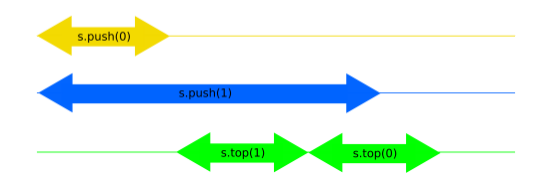
\includegraphics{t10f1.png}
\end{center}

\begin{itemize}
\item  Indica si la historia es linearizable

No, no es linerarizable, supongamos que si, tenemos entonces que:\\
$s.push(0) \leftarrow s.top(1) $ \\ 
pero sabemos que $s.push(1) \leftarrow s.top(1) $ \\
por lo tanto, $s.push(1)$ sucedio despues de $s.push(0)$\\
pero $s.top(1) \leftarrow s.top(1) $ lo cual es una contradicción, y por lo tanto no es linerizable $\blacksquare$ 

\item Indica si la historia es secuencialmente consistente.
Si lo es, como se muestra en el ordenamiento dado en la siguiente figura.
\begin{center}
  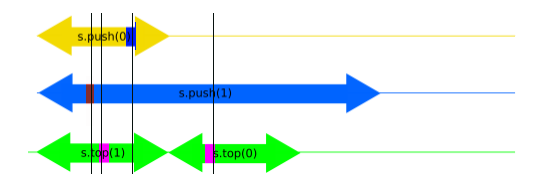
\includegraphics{t10f2.png}
\end{center}

\end{itemize}

\item[\bf{Problema 3}] Considera el siguiente código.\\
La clase {\tt AtomicInteger} es un contenedor para un valor entero. Esta clase contiene el método {\tt boolean CompareAndSet(int expect, int update)} que compara el valor actual del objeto con {\tt expect}. Si los valores son iguales, entonces atómicamente se reemplaza el valor del objeto con el valor update y se devuelve true. Si los valores no son iguales, el objeto no cambia y se regresa false. La clase también contiene el método {\tt int get()} que regresa el valor actual del objeto.\\
El código muestra la implementación de una cola FIFO. La cola guarda a los elementos en el arreglo items, el cual supondremos que tiene capacidad ilimitada; también contiene dos campos de la clase {\tt AtomicInteger}. head que es el índice de la casilla del siguiente elemento a ser eliminado y tail que es el índice de la casilla en la que se guardará el siguiente elemento. 
\newpage

\lstset{frame=tb,
  language=Java,
  aboveskip=3mm,
  belowskip=3mm,
  showstringspaces=false,
  columns=flexible,
  basicstyle={\small\ttfamily},
  numbers=left,
  numberstyle=\tiny\color{gray},
  keywordstyle=\color{blue},
  commentstyle=\color{dkgreen},
  stringstyle=\color{mauve},
  breaklines=true,
  breakatwhitespace=true
  tabsize=3
}
\begin{lstlisting}
class IQueue<T> f{
  AtomicInteger head = new AtomicInteger(0);
  AtomicInteger tail = new AtomicInteger(0);
  T[] items = (T[]) new Object[Integer.MAX_VALUE];
  public void enq(T x){
    int slot ;
    do{
      slot = tail.get () ;
    }while (! tail.compareAndSet(slot, slot + 1));
    items[slot] = x;
  }

  public T deq() throws EmptyException{
    T value;
    int slot ;
    do{
      slot = head.get() ;
      value = items[slot];
      if (value == null){
        throw new EmptyException();
      }
    }while(!head.compareAndSet(slot, slot + 1));
    return value;
  }
}
\end{lstlisting}

\begin{center}
  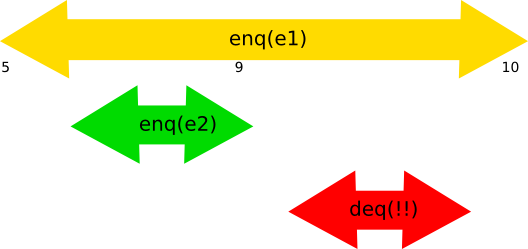
\includegraphics[width=300px]{t10f3.png}
\end{center}
Observe la ejecucion mostrada en el dibujo, los números debajo del hilo 1 representa que linea de código ya completo en ese momento.\\

El problema es que las operaciones {\tt tail.compareAndSet} y {\tt items[slot]=x} no son atómicas.\\
Así, en la ejecución mostrada cuando el hilo 3 empieza el hilo 1 ya ejecuto {\tt tail.compareAndSet} pero no ha ejecutado {\tt items[slot]=x}, por lo tanto {\tt 19.  value==null} será cierto y lanzada la excepción.\\

Así, la secuencia no es linearizable, pues si lo fuera, como el hilo 2 se ejecuta totalmente antes de que el hilo 3 empieze, el hilo 3 debería de tener disponible en la cola al menos el valor del hilo 2 y no regresar una excepción.

\end{enumerate}
\end{document}
